\chapter{Methodology} \label{sec:methodology}

As illustrated in Fig. \ref{fig:tikz_methodology}, we have our initial dataset that we split in :
\begin{itemize}
    \item a \textbf{validation set} (10\% of the dataset) used for hyper-parameter optimization or model selection for localisation and classification
    \item a \textbf{train / test set} (remaining dataset) used for the localisation and classification. The train set is used to learn the parameters of a classifier that is then evaluated on the test set (using the same dataset for learning and testing would lead to overfit the dataset and will not represent the capacity of the method to recognise new unknown element)
\end{itemize}

\begin{figure}[h]
    \centering
    \tikzstyle{block} = [rectangle, draw, text width=3cm, text centered, rounded corners,  fill=blue!20]
    \tikzstyle{line} = [draw,thick, -latex']
    \tikzstyle{cloud} = [draw, ellipse, text width=3cm, text centered]
    \tikzstyle{edge from parent}=[->,thick,draw]
    \begin{tikzpicture}[auto, edge from parent fork down]
        % Distance between node
        \tikzstyle{level 1}=[sibling distance=80mm,level distance=10ex]
        
        % Place nodes
        \node [cloud, fill=red!10] (base) {Dataset}
        child{node [cloud, fill=green!10] (validation) {Validation set}
            child{node [block, fill=blue!10] (hyperparameter) {Hyper-parameter optimization}}
        }
        child{node [cloud, fill=green!10] (train_test) {Train / test sets}
            child{node [block, fill=blue!10] (localisation) {Localisation}
                child {node[block, fill=blue!10](feature){Feature description}
                    child {node[block, fill=blue!10](classification){Classification}
                        child {node[block, fill=red!10](result){Result}
                        }
                    }
                }
            }
        };
        % Draw edges
        \path [line] (hyperparameter.east) -- (localisation.west);
        \path [line] (hyperparameter.south) -- (classification.west);
    \end{tikzpicture}
    \caption{General process of the localisation and classification}
    \label{fig:tikz_methodology}
\end{figure}

\section{Hyperparameter optimization}

There are numerous parameters that are part of the machine learning algorithm but are not learnt. Typical example include which kernel function used (if any) or the value of the penalty parameter $C$ for SVM, the number of $k$ of neighbourhoods for K-NN.

We use the exhaustive grid search method to select the parameters that have the highest performance score through 10 fold cross validation. It generates all the possible combination of parameters value and train / test the classifier.

\section{Localisation}

For localisation, a different approach from the literature has been used. The usual way is to detect area of food and non-food in a picture. Yet, it was noticed that the food items of UEC FOOD 256 and 100 tends to be in the middle and stands out. Moreover, requesting the user to take pictures that follow these characteristics is reasonable.

That's why a pre-trained CNN used for saliency detection has been used. It has been pre-trained in \cite{zhang2015SOD} on multiple datasets (Multi-Salient-Object, ILSVRC14). It is available on this gist \footnote{\url{https://gist.github.com/jimmie33/339fd0a938ed026692267a60b44c0c58}}.

The CNN structure is a copy of \enquote{GoogleNet} model \cite{Szegedy2015}, i.e. it is composed of 22 layers, corresponding to a succession of convolutional, max pooling and activation layers, the last one being a sigmoid function.

The CNN has been pre-trained to detect the likelihood to belong to one of the 100 arbitrary bounding boxes as presented in Fig. \ref{fig:seg_100_bboxes}.

\begin{figure}
    \centering
    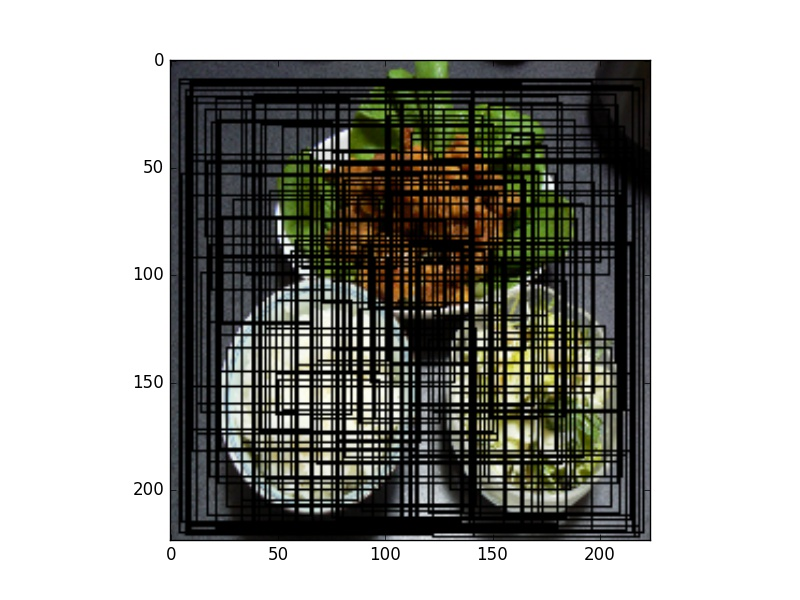
\includegraphics[scale=0.5]{img/seg_100_bboxes.jpg}
    \caption{Picture of the 100 possible bounding boxes that the salient CNN will try to recognise}
    \label{fig:seg_100_bboxes}
\end{figure}

Bounding boxes with a probability higher than a threshold $T$ are selected as candidate (if no box meet this limit, the bounding box with the maximum value is selected). As can be seen in figure \ref{fig:seg_97}, it generates a lot of overlapping copies. That's why, the final step of the localisation process is to discard small bounding boxes and overlapping ones (overlap higher than 30\%), keeping the ones with highest probabilities.

\begin{figure}
    \centering
    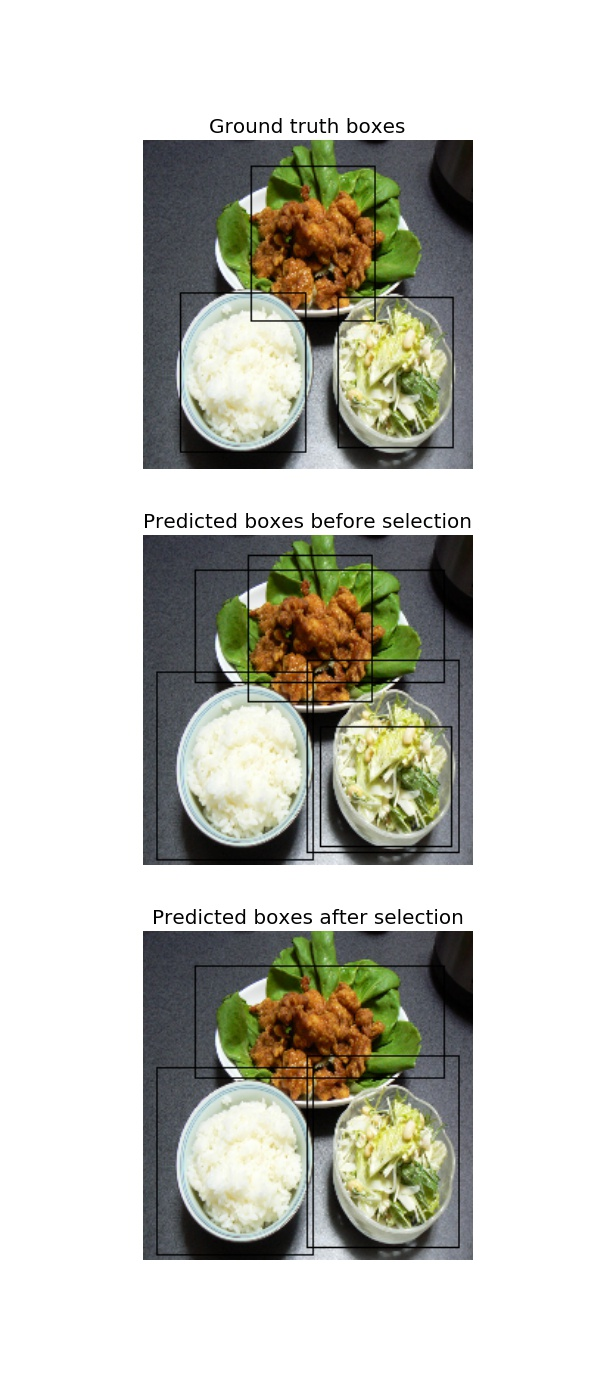
\includegraphics[height=20cm]{img/seg_97.jpg}
    \caption[Segmentation result]{Segmentation process with: the bounding boxes (top), the candidate bounding boxes (middle), the proposed bounding boxes after overlapping suppression (bottom)}
    \label{fig:seg_97}
\end{figure}

\section{Food recognition}
\subsection{Histograms and moments}

The first feature descriptor used a combination of LBP histogram with colour moments and histogram for each picture:
\begin{enumerate}
    %\item extract the sub-image delimited by the bounding box
    %\item resize this sub-image to $224 \times 224$ pixels
    \item extract a 100-bin histogram of local binary pattern on the grey scale image
    \item extract a 30-by-30-bin joint colour histogram for the channel $H$ and $s$ of the HSV  representation
    \item extract the first two moments of the R, G, B, H, S and Gray channels
    \item extract the 7 Hu moments
\end{enumerate}

The feature vectors are then normalized to have all features centred around zero (mean equal to 0) and have unit variance (equal to 1).

Then, multiple classifiers are applied :
\begin{itemize}
    \item decision tree
    \item random forest (made up of 500 trees)
    \item SVM
\end{itemize}

% Talk in result: show the best amelioration with hyperparemeter (but in general it only improve it by one or two percents) ??

\subsection{Bag of words}

The usual process of Bag-of-Features is used:
\begin{enumerate}
    \item detection of keypoints using a dense grid
    \item Root SIFT description
    \item clustering using the k-means algorithm to obtain a 1000-word codebook.
\end{enumerate}

Then, for each picture, we compute the histogram of occurrence counts of visual words. This descriptor is used with the SVM classifier and additive $\chi$-squared kernel.

\subsection{CNN as a Descriptor}

As described in section \ref{sec:classifier}, a CNN can be used as a feature descriptor. The pre-trained CNN was used for image recognition on ImageNet Challenge 2014 and presented in  \cite{Simonyan2014}. It is available on gist  \footnote{\url{https://gist.github.com/ksimonyan/3785162f95cd2d5fee77/}} .

The model is an improved version of the 19-layer model used by the VGG team in the ILSVRC-2014 competition. As the CNN used for segmentation, it takes a $224 \times 224$ RGB picture as input.

The output of the layer just before the FC is used as a descriptor. Thus, each picture is described by a 4096 feature vectors.

\section{Code}

The code is freely available on Github\footnote{\url{https://github.com/bnogaret/food_log}}.

I'm using python 3.5.2 and its scientific stack based on Scipy \cite{Oliphant2007}:
\begin{itemize}
    \item Numpy \cite{VanDerWalt2011} for N-dimensional array
    \item Pandas \cite{McKinney2010} for the data structure
    \item Scikit-image \cite{VanderWalt2014} and OpenCV 3 \cite{Bradski2000} for some of the image processing algorithms
    \item Scikit-learn \cite{Pedregosa2012} for most of the machine learning and Caffe \cite{Jia2014a} for the convolutional neural netzork framework
    \item Matplotlib \cite{Hunter2007} for 2D graph generation
    \item Sphinx for the documentation
\end{itemize}
